\subsection{题目描述}
Sketch the function \boldmath\(x^3 - 5x + 3 = 0\)\unboldmath
\begin{enumerate}
    \item[(i)] Determine the two positive roots to 4 decimal places using the bisection method.\\
          \textbf{Note:} You first need to bracket each of the roots.

    \item[(ii)] Take the two roots that you found in the previous question (accurate to 4 decimal places) and ``polish them up" to 14 decimal places using the Newton-Raphson method.

    \item[(iii)] Determine the two positive roots to 14 decimal places using the hybrid method.
\end{enumerate}

\subsection{程序描述}
标准的求根问题,顺便练习一下C++. 先使用Mathematica\textsuperscript{\textregistered}画出函数草图如下:
\begin{figure}[H]
    \centering
    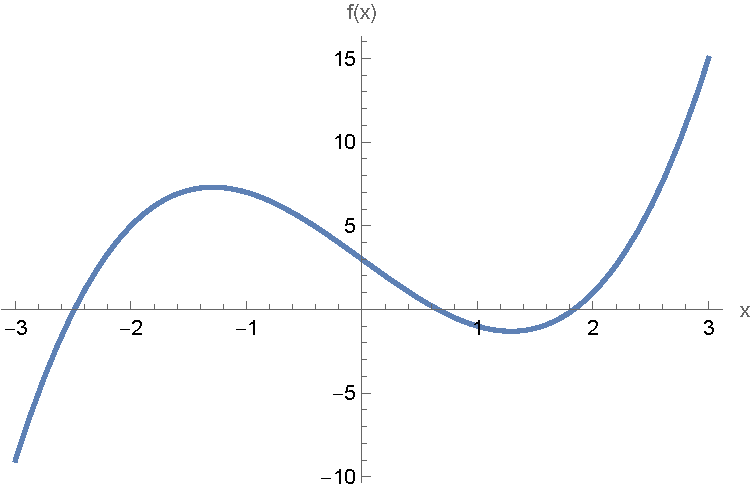
\includegraphics[width=0.6\textwidth]{Problem_1/Figs/1_plot.pdf}  % 调整图片宽度
    \caption{Plot of $x^3 - 5x + 3 = 0$.}
\end{figure}
\noindent 发现有两个正根,分别在$[0, 1]$和$[1, 2]$之间,有点好奇二分法的迭代,便先用Python写一下二分法的动态过程,见\texttt{./Codes/Problem_1/bisection\_visual.py},
使用\Colorbox{cmdbg}{\lstinline[language=bash]|python -u bisection_visual.py|}可以交互运行(需要安装\texttt{matplotlib,numpy}库)。运行后有三个选项,分别是前两个正根的查找与自定义区间查找,可以自行选择。

\texttt{./Codes/Problem_1/}中还有C++实现的二分法、牛顿法、混合法、Brent法与Ridder法,算法实现集成在了\texttt{methods.cpp}中,\texttt{main.cpp}负责封装与交互,\texttt{plotting.cpp}用ASCII绘制了草图,\texttt{functions.cpp}里面存储了本题函数与导数,拎出来是为了便于灵活测试其它函数,\texttt{utils.cpp}里面有两个工具函数,分别负责按照题目三小问的顺序输出结果与对比测试各类方法在三个根上的表现。
使用\Colorbox{cmdbg}{\lstinline[language=bash]|g++ *.cpp -o main|}编译,\Colorbox{cmdbg}{\lstinline[language=bash]|./main|}运行(也有已经编译好的\texttt{main.exe}),按照提示可以选择各类方法或者一起比较,也可以自定义查找区间与容差等参数。

原本对求根问题的兴趣不太大,至少没有24点那么有趣。在翻阅徐老师给的那本\textit{Numerical Recipe}的时候,发现虽然出了\href{https://numerical.recipes/book.html}{第三版},但出版商给每个章节都加弹窗广告。\textit{是可忍孰不可忍,我对金力发誓,绝不向校图书馆荐购它。}但里面提到的当下最常用的\href{https://github.com/scipy/scipy/blob/v1.14.1/scipy/optimize/_zeros_py.py#L679-L807}{Brent法}与\href{https://github.com/scipy/scipy/blob/v1.14.1/scipy/optimize/_zeros_py.py#L581-L676}{Ridder法}还是挺有意思的,在\texttt{scipy}里面也有它们的C语言实现,不过感觉写得没有\texttt{GNU Scientific Library}里面的清晰易懂,照猫画虎,在GPT的大力支持下,我用C++实现了一遍,最繁琐的的处理用户输入输出任务主要是它干的,想到了很多我没想到的细节,出色的前端工程师(bushi)!

Ridder法源自割线法和虚位法一脉。这一派的祖制是假设局部近似线性,因而在处理导数变化较大的地方表现不佳,尤其是割线法,虽号称有着黄金比率$1.618$的超线性收敛阶数,但在许多场合还不如二分法。新生代Ridder法就是变换一下$h(x)=f(x)\mathrm{e}^{ax}$,用一个指数因子来模拟潜在的非线性行为
\[
    e^{a(x_1-x_0)}=\frac{f(x_1)-\mathrm{sign}[f(x_0)]\sqrt{f(x_1)^2-f(x_0)f(x_2)}}{f(x_2)}.
\]
在此基础上再使用虚位法,考虑到这个指数函数的查找提供的二阶加速,以及本身多一次的计算,其理论收敛指数为$\sqrt{2} \approx 1.414 < 1.618$,but who cares about theory? 实际效果还是不错的,详情参见\ref{alg:ridder_method}。

Brent法的核心思想继承自Dekker法,后者与我们题目第三问提示的Hybrid法有些类似,但在局部加速收敛的过程中,用的不是基于导数的Newton法,而是用割线法,也即在小区间内倾向于使用单点迭代,但在迭代点越过区间范围时使用二分法补救,非常自然且优美的思路。Brent主要是在Dekker法的基础上加入了逆二次插值,顾名思义,就是在局部二次拟合反函数$x(y)$,用的方法也很暴力,高数书上的拉格朗日插值:
\[
    x=\frac{\left[y-f\left(x_{1}\right)\right]\left[y-f\left(x_{2}\right)\right]x_{3}}{\left[f\left(x_{3}\right)-f\left(x_{1}\right)\right]\left[f\left(x_{3}\right)-f\left(x_{2}\right)\right]}+\frac{\left[y-f\left(x_{2}\right)\right]\left[y-f\left(x_{3}\right)\right]x_{1}}{\left[f\left(x_{1}\right)-f\left(x_{2}\right)\right]\left[f\left(x_{1}\right)-f\left(x_{3}\right)\right]}+\frac{\left[y-f\left(x_{3}\right)\right]\left[y-f\left(x_{1}\right)\right]x_{2}}{\left[f\left(x_{2}\right)-f\left(x_{3}\right)\right]\left[f\left(x_{2}\right)-f\left(x_{1}\right)\right]}.
\]
听起来好像没有很高大上,但Brent的神来之笔在于,考虑到了实际过程中的rounderror问题,譬如在三个点的拟合时,如果其中两个的函数值本身就接近,会导致拟合效果很差(脑补一下对直线进行水平轴抛物线拟合的糟糕后果),所以对是否返回二分法进行了详细的分类讨论,详情参见\ref{alg:brent_method}。原版Brent还引入了一些中间变量来减少舍入误差,两年后还提出来用双曲外推替代二次插值,我就没继续学习了。

\subsection{伪代码}
\begin{algorithm}[H]
    \caption{Bisection Method}
    \label{alg:bisection}
    \KwIn{$a$, $b$ (long double), \texttt{tol} (long double), \texttt{max\_iter} (int)}
    \KwOut{$c$ (long double) \tcp*[r]{Approximate root}}

    \For{$i \gets 1$ \textbf{to} \texttt{max\_iter}}{
        $c \gets \dfrac{a + b}{2}$\tcp*[r]{Compute midpoint}
        \If{$|b - a| < \texttt{tol}$}{
            \Break\tcp*[r]{Convergence achieved}
        }
        \If{$f(a) \cdot f(c) < 0$}{
            $b \gets c$\tcp*[r]{Update interval}
        }\Else{
            $a \gets c$\tcp*[r]{Update interval}
        }
    }
    \Return $c$
\end{algorithm}

\vspace{5pt}
\begin{algorithm}[H]
    \caption{Newton-Raphson Method}
    \label{alg:newton_raphson}
    \KwIn{$x_0$ (long double), \texttt{tol} (long double), \texttt{max\_iter} (int)}
    \KwOut{$x$ (long double) \tcp*[r]{Approximate root}}

    \For{$i \gets 1$ \textbf{to} \texttt{max\_iter}}{
        \If{$f'(x_0) = 0$}{
            \RaiseError "Derivative zero"\;
        }
        $x \gets x_0 - \dfrac{f(x_0)}{f'(x_0)}$\tcp*[r]{Compute next approximation}
        \If{$|x - x_0| < \texttt{tol}$}{
            \Break\tcp*[r]{Convergence achieved}
        }
        $x_0 \gets x$\tcp*[r]{Update current value}
    }
    \Return $x$
\end{algorithm}



\begin{algorithm}[H]
    \caption{Hybrid Method}
    \label{alg:hybrid_method}
    \KwIn{$a$, $b$ (long double), \texttt{tol} (long double), \texttt{max\_iter} (int)}
    \KwOut{$c$ (long double) \tcp*[r]{Approximate root}}

    \For{$i \gets 1$ \textbf{to} \texttt{max\_iter}}{
        $c \gets \dfrac{a + b}{2}$\tcp*[r]{Compute midpoint}
        \If{$\dfrac{b - a}{2} < \texttt{tol}$}{
            \Break\tcp*[r]{Convergence achieved}
        }
        \If{$f'(c) \ne 0$ \textbf{and} $d = c - \dfrac{f(c)}{f'(c)}$ is in $(a, b)$}{
            \If{$|d - c| < \texttt{tol}$}{
                \Return $d$\tcp*[r]{Convergence achieved}
            }
            \If{$f(a) \cdot f(d) < 0$}{
                $b \gets d$\tcp*[r]{Update interval}
            }\Else{
                $a \gets d$\tcp*[r]{Update interval}
            }
            \Continue\tcp*[r]{Proceed to next iteration}
        }
        \If{$f(a) \cdot f(c) < 0$}{
            $b \gets c$\tcp*[r]{Update interval (Bisection)}
        }\Else{
            $a \gets c$\tcp*[r]{Update interval (Bisection)}
        }
    }
    \Return $c$
\end{algorithm}

\begin{algorithm}[H]
    \caption{Brent's Method}
    \label{alg:brent_method}
    \KwIn{$a$, $b$, \texttt{tol} (long double), \texttt{max\_iter} (int), \texttt{decimal\_places} (int)}
    \KwOut{$root$ (long double) \tcp*[r]{Approximate root}}

    \If{$f(a) \cdot f(b) \geq 0$}{
        \RaiseError{"Brent's method fails. f(a) and f(b) should have opposite signs."}\;
    }

    \If{$|f(a)| < |f(b)|$}{
        Swap $a \leftrightarrow b$\tcp*[r]{Ensure $a$ corresponds to the larger $|f(x)|$}
    }

    $c \gets a$, $s \gets b$, \texttt{mflag} $\gets$ True\tcp*[r]{Initialize $c$, $s$, and set bisection flag}

    \For{$i \gets 1$ \textbf{to} \texttt{max\_iter}}{
        \If{$f(b) \neq f(c)$ \textbf{and} $f(a) \neq f(c)$}{
            $s \gets \dfrac{a \cdot f(b) \cdot f(c)}{(f(a) - f(b)) \cdot (f(a) - f(c))} + \dfrac{b \cdot f(a) \cdot f(c)}{(f(b) - f(a)) \cdot (f(b) - f(c))} + \dfrac{c \cdot f(a) \cdot f(b)}{(f(c) - f(a)) \cdot (f(c) - f(b))}$\tcp*[r]{Inverse quadratic interpolation}
        }
        \Else{
            $s \gets b - f(b) \cdot \dfrac{b - a}{f(b) - f(a)}$\tcp*[r]{Secant method step}
        }

        \If{$s < \dfrac{3a + b}{4}$ \textbf{or} $s > b$ \textbf{or} (\texttt{mflag} \textbf{and} $|s - b| \geq |b - c| / 2$) \textbf{or} (\textbf{not} \texttt{mflag} \textbf{and} $|s - b| \geq |c - d| / 2$) \textbf{or} (\texttt{mflag} \textbf{and} $|b - c| < \texttt{tol}$) \textbf{or} (\textbf{not} \texttt{mflag} \textbf{and} $|c - d| < \texttt{tol}$)}{
            $s \gets \dfrac{a + b}{2}$, \texttt{mflag} $\gets$ True\tcp*[r]{Bisection step for stability}
        }
        \Else{
            \texttt{mflag} $\gets$ False \tcp*[r]{Use interpolation or secant step}
        }

        $c \gets b$, $f(c) \gets f(b)$ \tcp*[r]{Update $c$ and prepare next iteration}

        \If{$f(a) \cdot f(s) < 0$}{
            $b \gets s$\tcp*[r]{Set new upper bound}
        }
        \Else{
            $a \gets s$\tcp*[r]{Set new lower bound}
        }

        \If{$|f(a)| < |f(b)|$}{
            Swap $a \leftrightarrow b$\tcp*[r]{Ensure $|f(a)| \geq |f(b)|$ for stability}
        }

        \If{$|b - a| < \texttt{tol}$}{
            \Break\tcp*[r]{Convergence achieved within tolerance}
        }
    }

    \Return $b$\;
\end{algorithm}


\begin{algorithm}[H]
    \caption{Ridder's Method}
    \label{alg:ridder_method}
    \KwIn{$a$, $b$ (long double), \texttt{tol} (long double), \texttt{max\_iter} (int)}
    \KwOut{$x$ (long double) \tcp*[r]{Approximate root}}

    \For{$i \gets 1$ \textbf{to} \texttt{max\_iter}}{
    $c \gets \dfrac{a + b}{2}$\tcp*[r]{Compute midpoint}
    $s \gets \sqrt{f(c)^2 - f(a) f(b)}$\;
    \If{$s = 0$}{
        \Return $c$\tcp*[r]{Convergence achieved}
    }
    $sign \gets \operatorname{sgn}(f(a) - f(b))$\tcp*[r]{Determine sign}
        $x \gets c + (c - a) \dfrac{f(c)}{s} \cdot sign$\tcp*[r]{Compute new approximation}
        \If{$|f(x)| < \texttt{tol}$}{
            \Return $x$\tcp*[r]{Convergence achieved}
        }
        \If{$f(c) \cdot f(x) < 0$}{
            $a \gets c$, $b \gets x$\tcp*[r]{Update interval}
        }
        \ElseIf{$f(a) \cdot f(x) < 0$}{
            $b \gets x$\tcp*[r]{Update interval}
        }
        \Else{
            $a \gets x$\tcp*[r]{Update interval}
        }
        \If{$|b - a| < \texttt{tol}$}{
            \Break\tcp*[r]{Convergence achieved}
        }
        }
        \Return $\dfrac{a + b}{2}$
\end{algorithm}


\subsection{结果示例}
\begin{figure}[h]
    \centering
    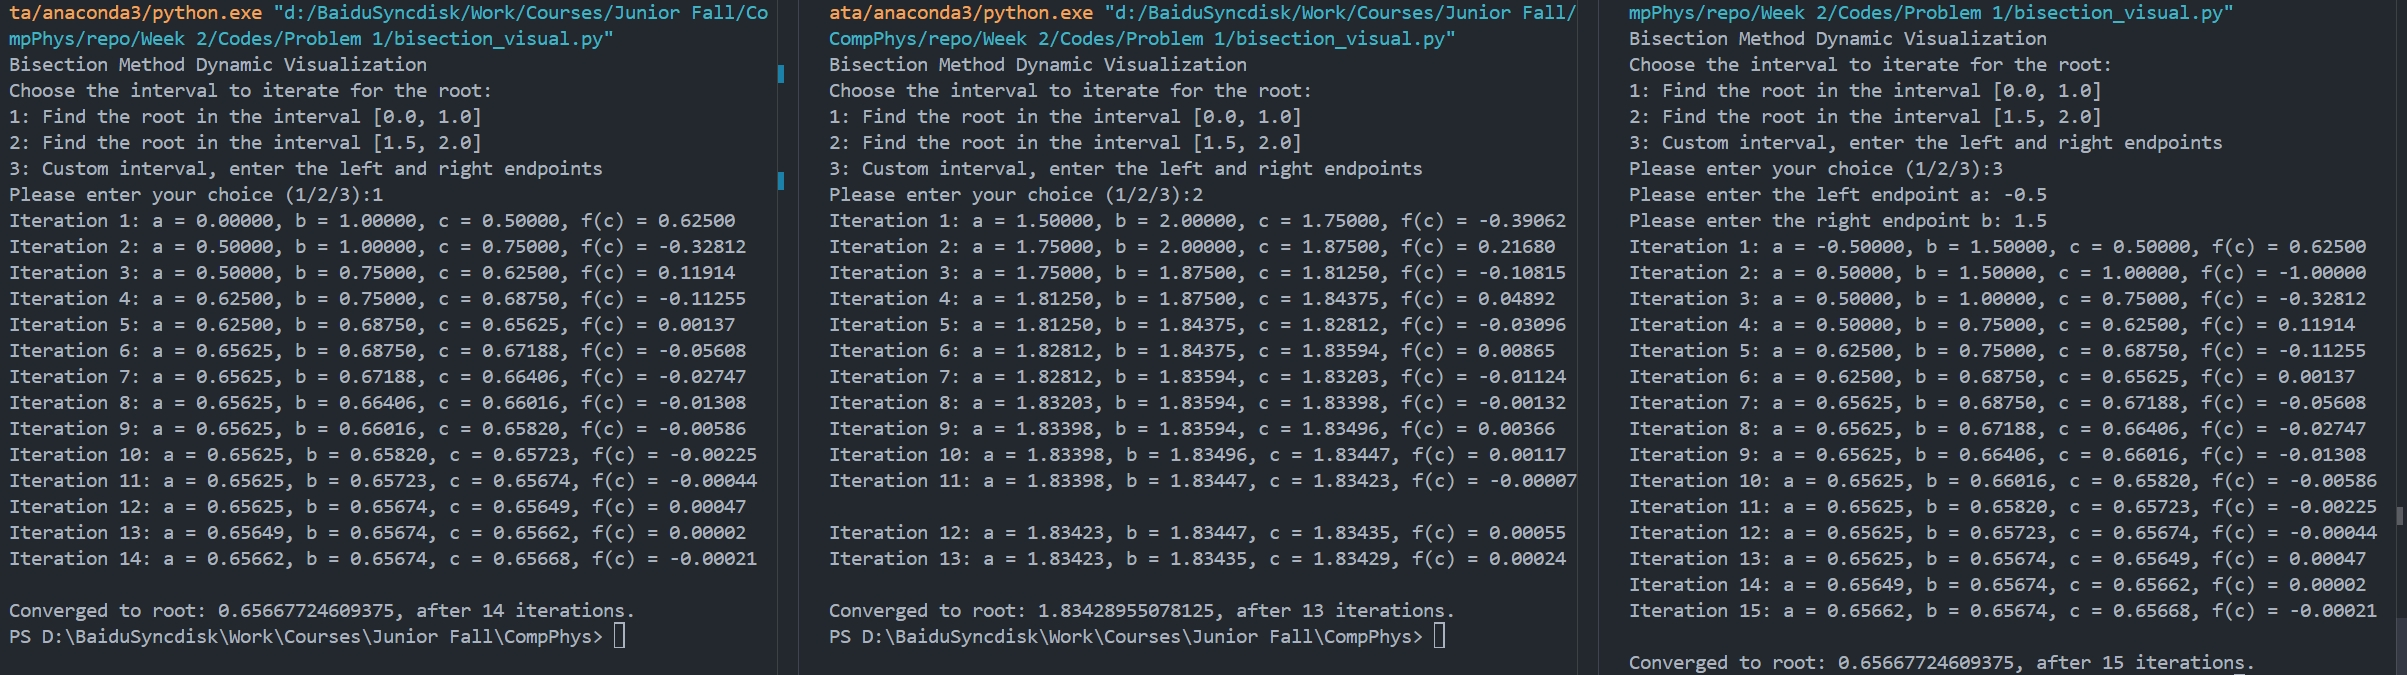
\includegraphics[width=1.0\textwidth]{Problem_1/figs/1_bisection.png}
    \caption{\texttt{bisection\_visual.py}三种选项对比}
    \label{fig:1_py_bisection}
\end{figure}

\begin{figure}[H]
    \centering
    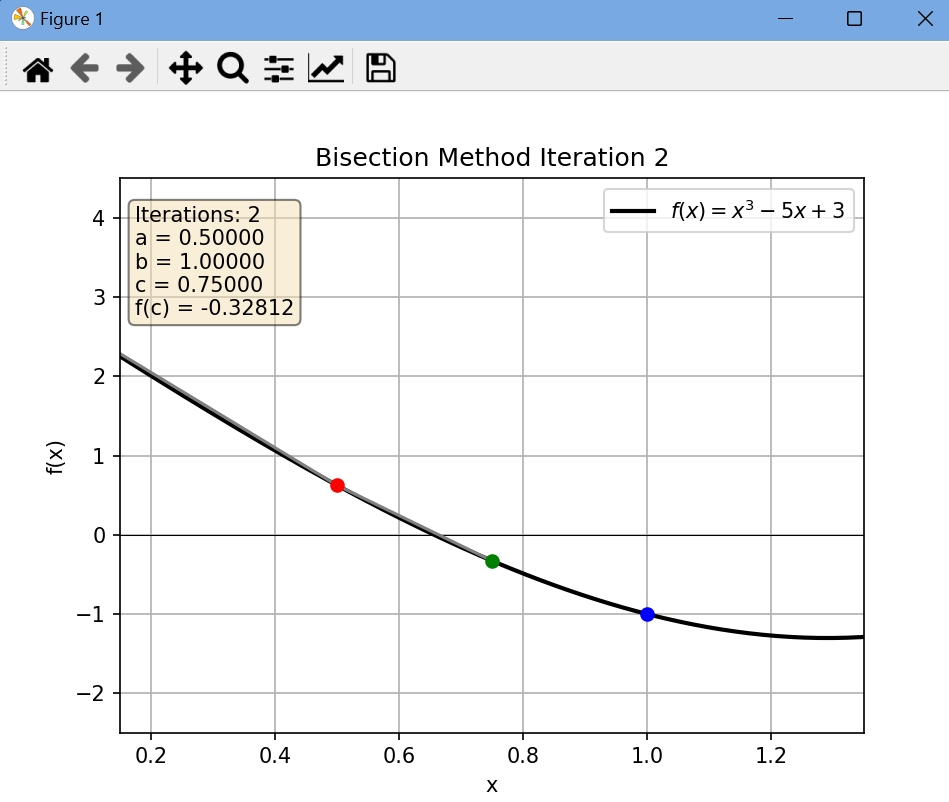
\includegraphics[width=0.6\textwidth]{Problem_1/Figs/1_animation.png}
    \caption{\texttt{bisection\_visual.py}动画示意}
    \label{fig:1_py_animation}
\end{figure}

\begin{figure}[H]
    \centering
    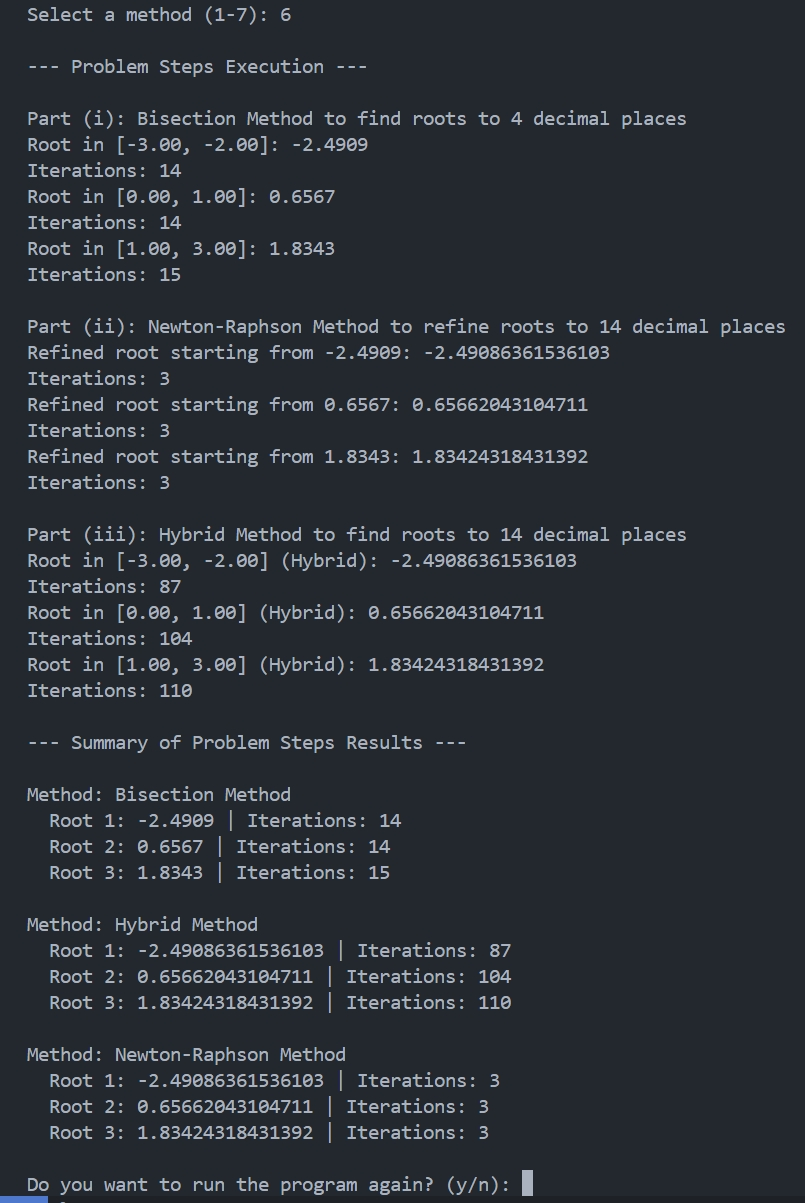
\includegraphics[width=0.7\textwidth]{Problem_1/Figs/1_step.png}
    \caption{\texttt{main.cpp}模式6,按题目顺序尝试三种方法}
    \label{fig:1_cpp_step}
\end{figure}

\begin{figure}[H]
    \centering
    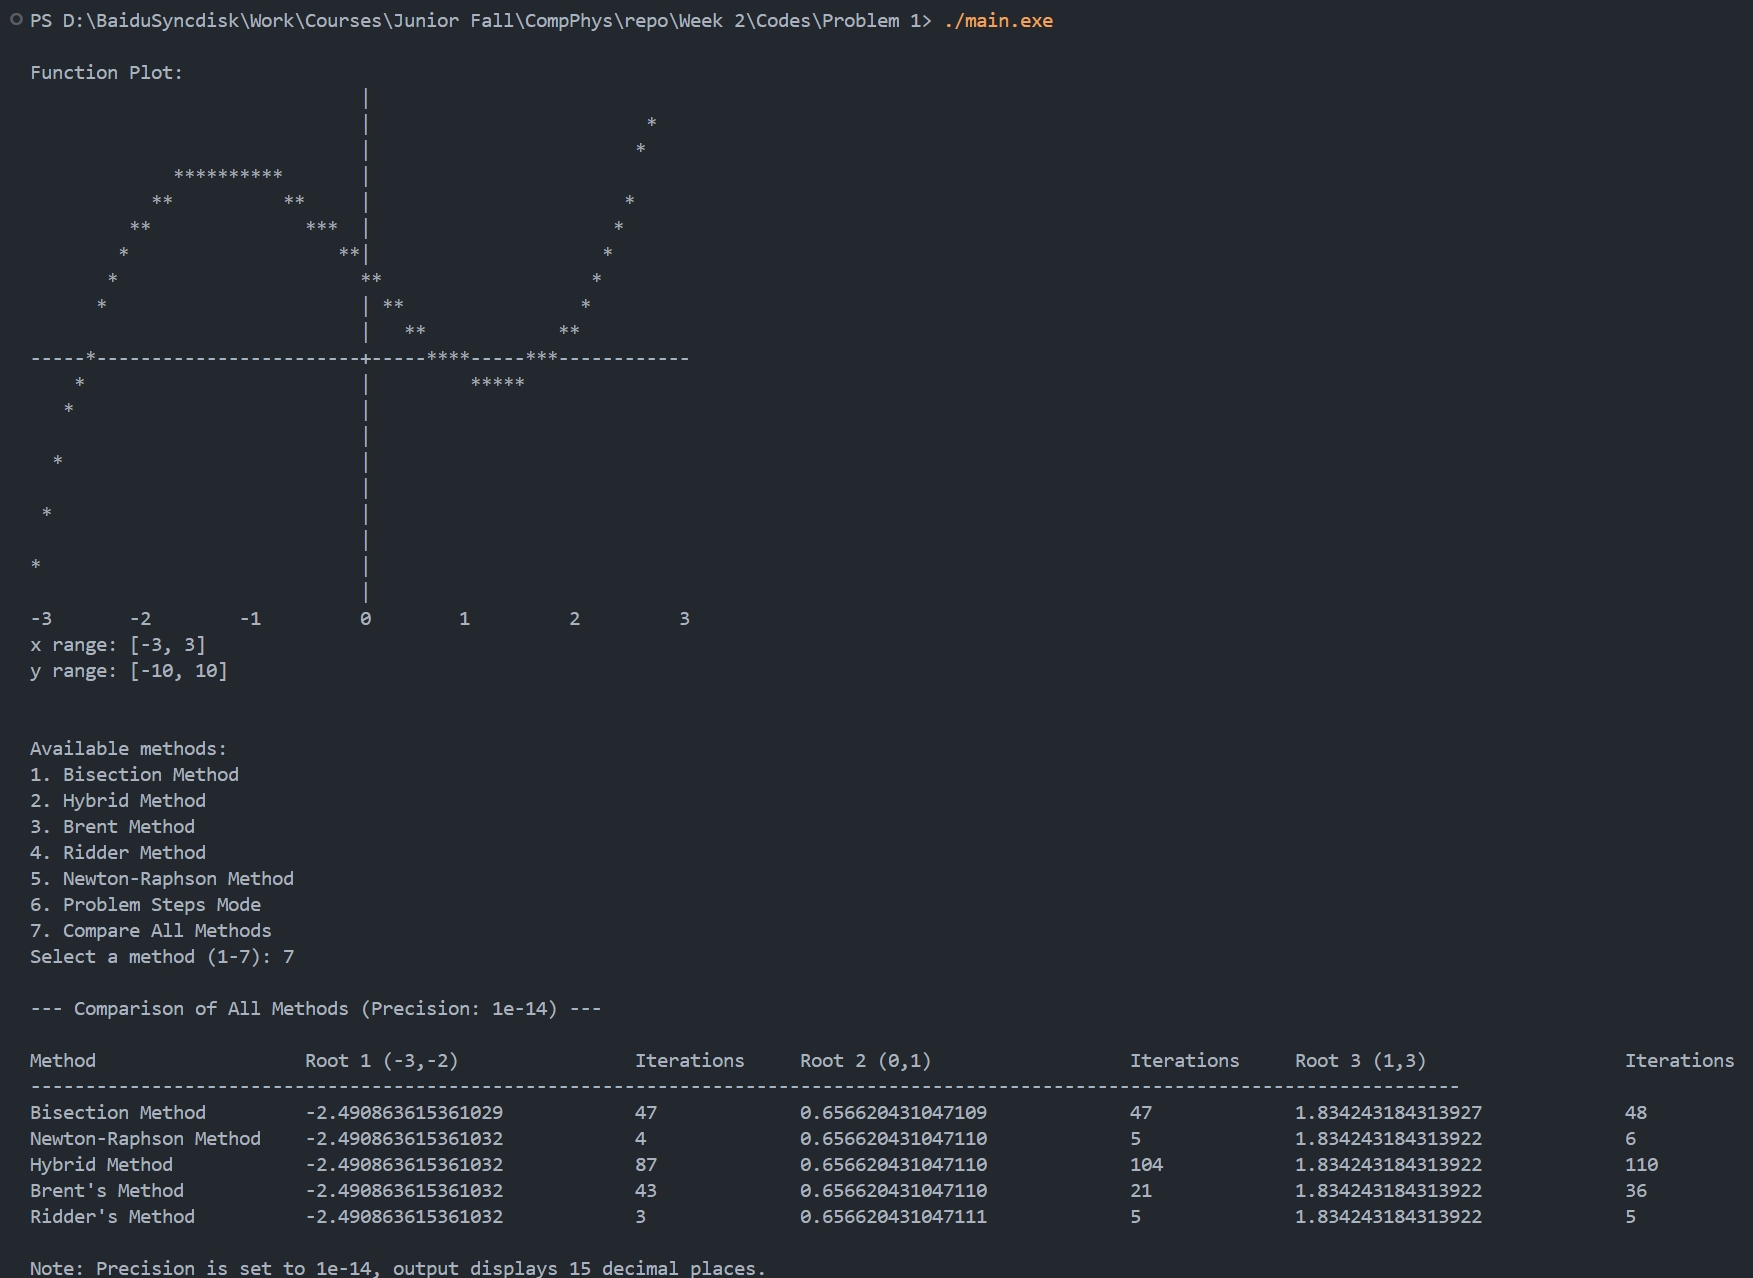
\includegraphics[width=1.0\textwidth]{Problem_1/Figs/1_all.png}
    \caption{\texttt{main.cpp}模式7,对比五种方法}
    \label{fig:1_cpp_all}
\end{figure}
